\documentclass{article}

\usepackage[margin=1in]{geometry}
\usepackage{amsmath}
\usepackage{amssymb}
\usepackage{graphicx}

\begin{document}

\title{M 476 - Homework 3}
\author{Nathan Stouffer}

\maketitle
\newpage

\section*{Problem 1}

Problem: Consider the map $f: \mathbb{R}^3 \to \mathbb{R}^2$, $(x,y,z) \to (3*x*y^2 + 1, 2*z^2)$. Deduce that $f$ is continuous by writing it as a composition of the functions we have previously proved to be continuous. \\\\
Solution: We first observe that $f$ is a projection form $\mathbb{R}^3 \to \mathbb{R}$. Let $g: \mathbb{R}^2 \to \mathbb{R}$, $(x,y) \to 3*x*y^2$ and $h: \mathbb{R}^2 \to \mathbb{R}$, $(x,z) \to 2*z^2 + x$. Then, by obs (prod), $f$ is continuous only if the components of $f$ are continuous. That is, $f$ is continuous if $g$ and $h$ are continuous. The functions $g$ and $h$ are continuous since they are composed of sums of products, which are continuous by obs (add) and obs (mult). The composition is shown in the image below.
\begin{figure}[h]
	\centering
	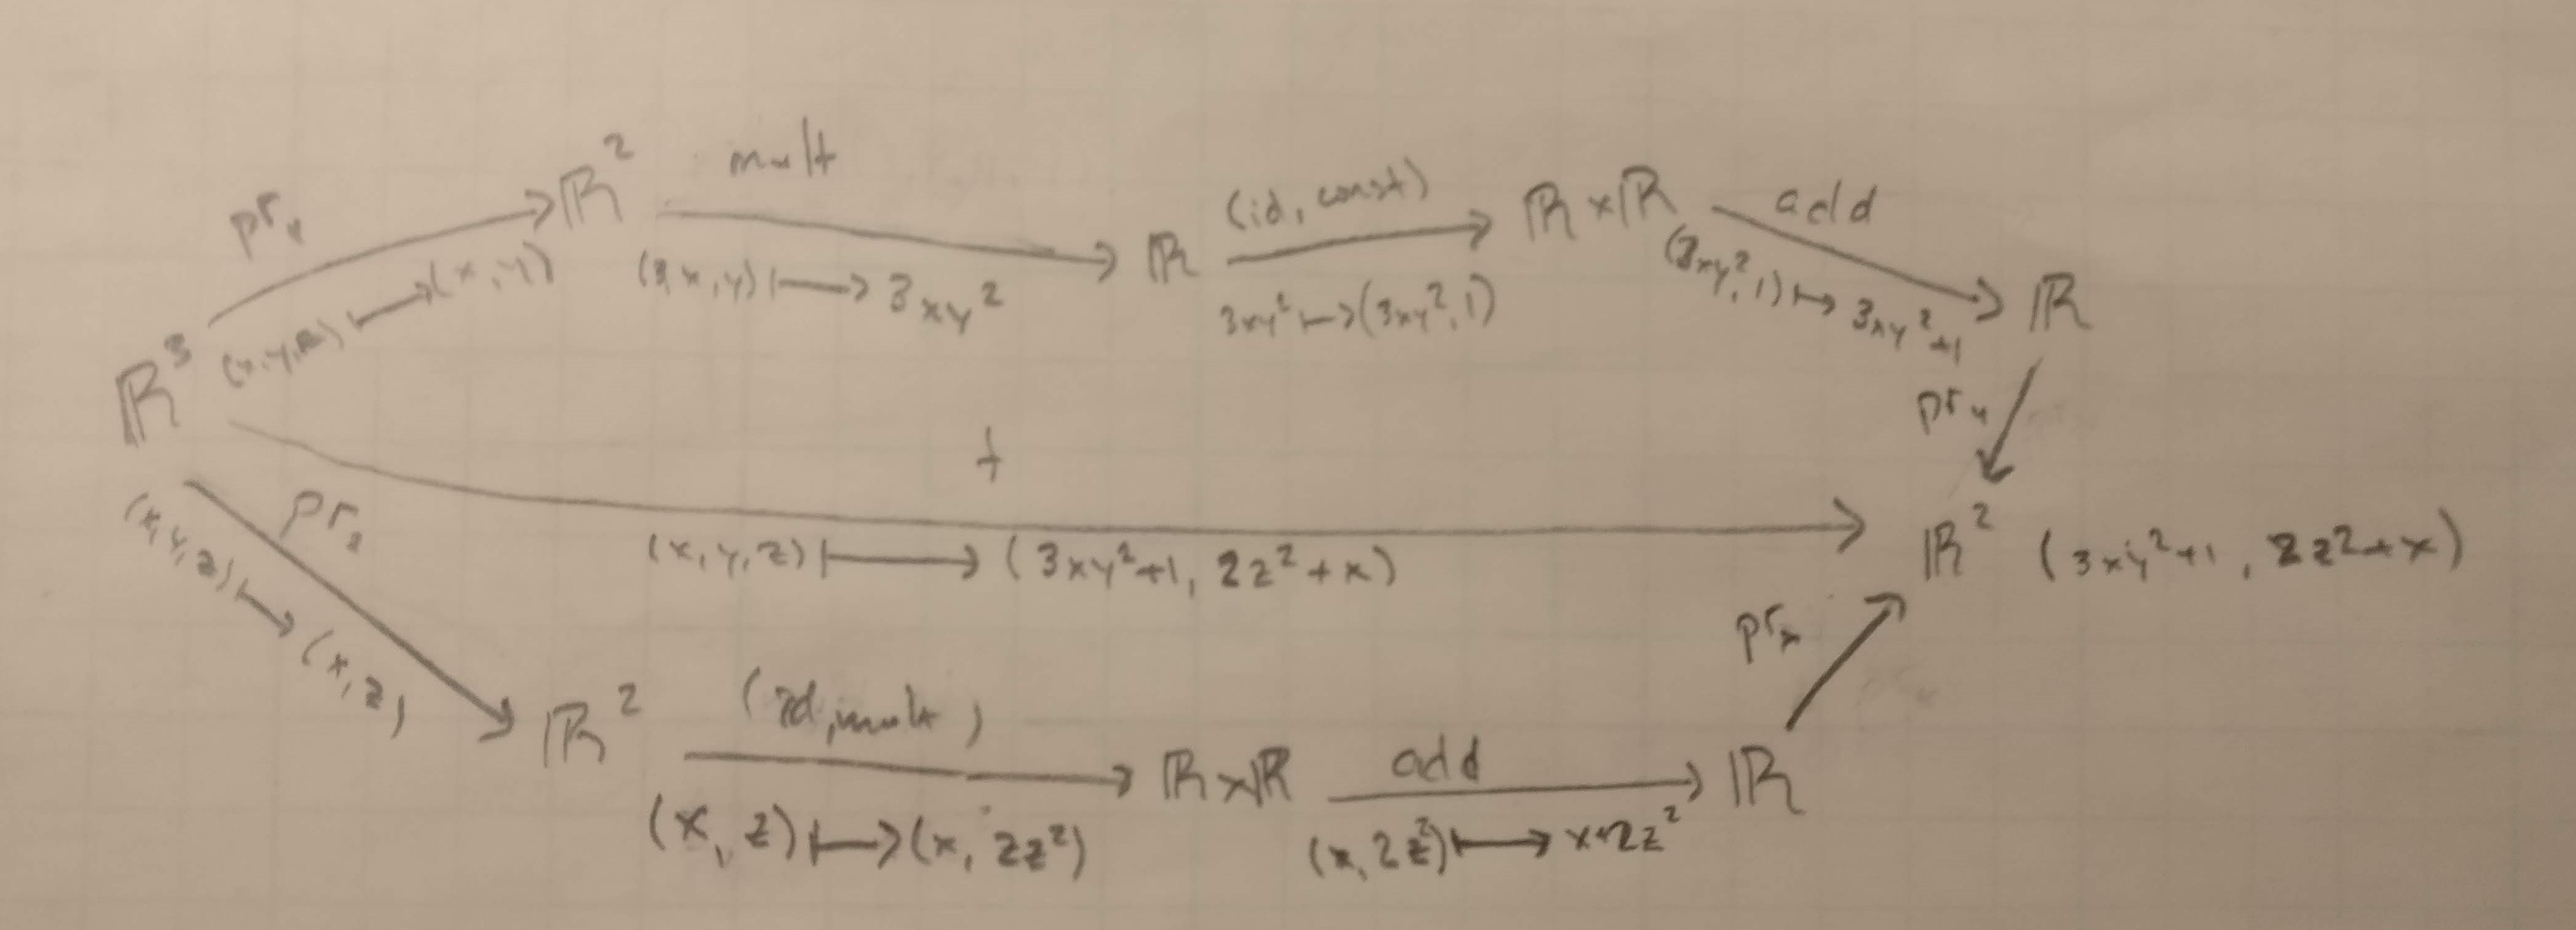
\includegraphics[width=4in]{composition-map}
\end{figure}

\newpage

\section*{Problem 2}

Problem: Let $X := \{ (x,y) \in \mathbb{R}^2 \mid x^2+y^2=1 \text{ and } y<1 \} \subset \mathbb{R}^2$ and let $Z := \{(x,y) \in \mathbb{R}^2 \mid y=0 \}$. Consider the map $f:X \to Z$ whose value on $(x,y)$ is the unique $(x^\prime , 0) \in Z$ for which the triple of points in $\mathbb{R}^2$
\begin{center}
	$\{(0,1), (x,y), (x^\prime, 0)\}$
\end{center}
are co-linear. Prove that there is indeed a unique such value $f(x,y)$ for each $(x,y) \in X$; prove that $f$ is continuous. \\\\
Solution: To prove that a unique $f(x,y)$ exists for each $(x,y)$ we must remember that the point $(x,y)$ must lie on the unit circle $C \setminus (0,1)$. Now, imagine the line defined by $(0,-1)$. This line intersects the x-axis at $(0,0)$. Moving $(x,y)$ along the unit circle when $x > 0$ will intersect all $x^\prime$ on the x-axis greater than 0 and moving $(x,y)$ along the unit circle when $x < 0$ will intersect all $x^\prime$ on the x-axis less than 0. \\\\
To construct the function $f$, we begin with the fact that the points $\{(0,1), (x,y), (x^\prime, 0)\}$ must be co-linear. Each of the three points lie on a line $L$ with slope $m = \dfrac{1 - y}{0 - x} = \dfrac{y - 1}{x}$. We also know that the y-intercept of $L$ is $(0, 1)$, which gives $L$ to be $b = \dfrac{y - 1}{x} * a + 1$ where $(a,b) \in \mathbb{R}^2$ is an ordered pair that satisfies $L$. Since the line $L$ must also intersect $(x^\prime , 0)$, we can substitute $(x^\prime , 0)$ in for $(a,b)$. Now $L$ is $0 = \dfrac{y - 1}{x} * x^\prime + 1$. Solving for $x^\prime$: $x^\prime = \dfrac{x}{1 - y}$. Thus, $f$ is given by $(x,y) \to (\dfrac{x}{1-y}, 0)$. \\\\
Now to prove that the function $f$ is continuous. The function $f$ is continuous if each of the components of $f(x,y)$ are continuous. The first component of $f$ is continuous since $\dfrac{x}{1 - y}$ is first made up of an addition and then a division, which are continuous by obs (add) and obs (div). Additionally, $y \neq 1$, so we will never divide by zero. The second component of $f$ is continuous for it is a constant mapping and constant maps are continuous by obs (const). Since the components of $f$ are continuous, the function $f$ must be continuous.

\newpage

\section*{Problem 3}

Problem: For $n \geq 0$, denote $\mathbb{S}^n := \{ (x_0, x_1, ..., x_n) \mid x_0^2 + x_1^2 + ... + x_n^2 = 1 \} \subset \mathbb{R}^{n+1}$. Prove that $\mathbb{S}^n$ is path-connected if and only if $n > 0$.\\\\
Solution: We will first show that if $\mathbb{S}^n$ is path-connected, then $n > 0$. This will be shown using the contrapositive of the statement: If $n \leq 0$, then $\mathbb{S}^n$ is not path-connected.
We can be more restrictive on our value for $n$ since $n \geq 0$, this implies that $n = 0$. Thus we now must show that following is true:
\begin{center}
	If $n = 0$, then $\mathbb{S}^n$ is not path-connected.
\end{center}
Now there is only one case: when $n = 0$, the set $\mathbb{S}^0 = \{ x_0 \mid x_0^2 = 1 \} = \{ -1, 1 \} \subset \mathbb{R}$. The individual elements $-1, 1 \in \mathbb{R}$ are not connected and the contrapositive is proved. Thus it is proved that if $\mathbb{S}^n$ is path-connected, then $n > 0$. \\\\
We will now show that if $n > 0$, then $\mathbb{S}^n$ is path-connected. Since $n > 0$, the set $\mathbb{S}^n \subset \mathbb{R}^{n+1}$ where the Euclidean Space is $\mathbb{R}^{n+1}$ is $\mathbb{R}^{2}$ or greater by definition of $\mathbb{S}^n$. 
Since we are at least in $\mathbb{R}^2$ or greater, it is possible to arbitrarily choose 2 distinct vectors $p,q \in \mathbb{S}^n$.
If we can construct a continuous path (beginning at $t = 0$ and ending at $t = 1$) from $p$ to $q$, we will have proven that $\mathbb{S}^n$ is path-connected.
Consider the map $\gamma : \mathbb{R} \to \mathbb{S}^n$, $t \to \cos (2\pi t) * p + \sin (2 \pi t) * q$.
Then, $\gamma (0) = p$ and $\gamma (1) = q$. So, now we must show that $\gamma$ is continuous.
The function $\gamma$ must be continuous for $\gamma$ is composed of the continuous functions $mult$, $sin$, and $cos$. Since $\gamma$ is continuous, $\mathbb{S}^n$ must be path connected.
Therefore, if $n > 0$, then $\mathbb{S}^n$ is path-connected. \\\\
Now we have shown that if $\mathbb{S}^n$ is path-connected, then $n > 0$ and that $n > 0$ implies that $\mathbb{S}^n$ is path-connected. Thus, it is true that $\mathbb{S}^n$ is path-connected if and only if $n > 0$.

\newpage

\section*{Problem 4}

Problem: Let $X \subset \mathbb{R}^n$ and $y \subset \mathbb{R}^k$. Prove that $X \times Y$ is path-connected if and only if both $X$ and $Y$ are path-connected. Deduce form this and the previous problem that the torus $\mathbb{S}^1 \times \mathbb{S}^1$ is path-connected. \\\\
Solution: To prove that $X \times Y$ is path-connected if and only if both $X$ and $Y$ are path-connected, we must first show that $X \times Y$ is path-connected $\implies$ both $X$ and $Y$ are path-connected and then prove that $X \times Y$ is path-connected $\impliedby$ both $X$ and $Y$ are path-connected. \\\\
We first note the following theorem: The continuous image of a path-connected subset of Euclidean Space is path-connected. Let this theorem be Theorem 1. \\\\
We now prove that $X \times Y$ is path-connected $\implies$ both $X$ and $Y$ are path-connected. We assume that $X \times Y$ is path-connected. By Theorem 1, we also know that the continuous image of a path-connected set is path-connected. The projection map is continuous by obs (proj). Without loss of generality, we choose to prove that $X$ is path-connected. To prove that $X$ is path-connected, define $f:X \times Y \to X$, $(x,y) \to (x)$. The function $f$ is continuous since it is a projection, and thus the image of $f$ is continuous. Since the image $X$ is continuous, $X$ must also be path connected by Theorem 1. Thus, $X$ and $Y$ must both be path-connected. \\\\
We will now show that both $X$ and $Y$ are path-connected $\implies$ $X \times Y$ is path-connected. Since $X$ and $Y$ are both path-connected, by Theorem 1, their image under a continuous function must also be path-connected. The product function is continuous by obs (prod), therefore, $X \times Y$ must be path-connected. \\\\
We now show that the torus $\mathbb{S}^1 \times \mathbb{S}^1$ is path-connected. Because of the proof in Problem 3, we know that $\mathbb{S}^n$ where $n=1$ is path-connected since $n > 0$. Additionally, the first part of Problem 4 proves that, given path-connected sets $A$ and $B$, the set $A \times B$ is also path-connected. Since a torus is a Cartesian product between two path-connected sets, a torus is also path connected.

\end{document}